\documentclass[10pt]{article}
\usepackage[paperwidth=198mm,paperheight=59mm,margin=1mm]{geometry}
\usepackage{newtxtext,newtxmath,tikz,pgfplots}
\pgfplotsset{compat=1.18}
\definecolor{methodblue}{HTML}{216A85}
\definecolor{controlgray}{HTML}{555555}
\definecolor{accentorange}{HTML}{A64B1D}
\pagestyle{empty}
\begin{document}\noindent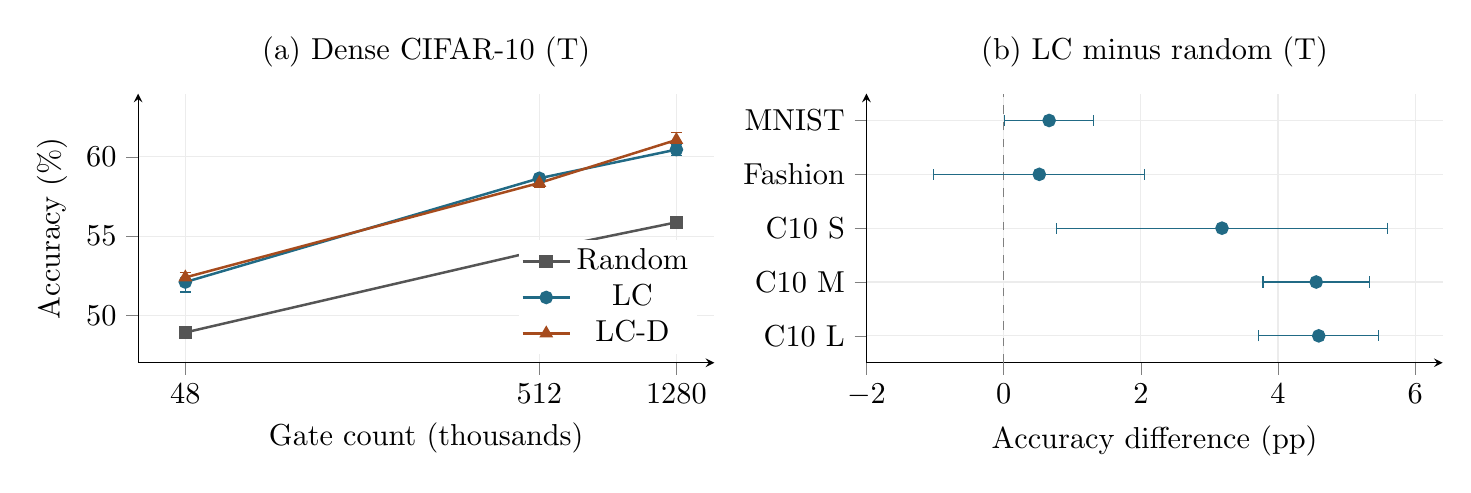
\begin{tikzpicture}
\begin{axis}[width=89mm,height=50mm,axis lines=left,tick align=outside,grid=major,grid style={gray!15},scaled ticks=false,tick label style={font=\fontsize{11}{13}\selectfont},label style={font=\fontsize{11}{13}\selectfont},title style={font=\fontsize{11}{13}\selectfont},legend style={font=\fontsize{11}{13}\selectfont,draw=none,fill=white,inner sep=1pt},title={(a) Dense CIFAR-10 (T)},xmode=log,log basis x=10,xmin=35,xmax=1650,ymin=47,ymax=64,xtick={48,512,1280},xticklabels={48,512,1280},xlabel={Gate count (thousands)},ylabel={Accuracy (\%)},legend pos=south east]
\addplot+[color=controlgray,mark=square*,mark size=2pt,line width=0.9pt,mark options={solid,fill=controlgray,draw=controlgray},error bars/.cd,y dir=both,y explicit] coordinates {(48,48.913332) +- (0,0.34588056)(512,54.096665) +- (0,0.17097752)(1280,55.869999) +- (0,0.30805842)};
\addlegendentry{Random}
\addplot+[color=methodblue,mark=*,mark size=2pt,line width=0.9pt,mark options={solid,fill=methodblue,draw=methodblue},error bars/.cd,y dir=both,y explicit] coordinates {(48,52.096665) +- (0,0.63042328)(512,58.653332) +- (0,0.16802787)(1280,60.463332) +- (0,0.34818579)};
\addlegendentry{LC}
\addplot+[color=accentorange,mark=triangle*,mark size=2pt,line width=0.9pt,mark options={solid,fill=accentorange,draw=accentorange},error bars/.cd,y dir=both,y explicit] coordinates {(48,52.389999) +- (0,0.29512717)(512,58.356665) +- (0,0.25324545)(1280,61.073332) +- (0,0.46285352)};
\addlegendentry{LC-D}
\end{axis}
\begin{axis}[width=89mm,height=50mm,axis lines=left,tick align=outside,grid=major,grid style={gray!15},scaled ticks=false,tick label style={font=\fontsize{11}{13}\selectfont},label style={font=\fontsize{11}{13}\selectfont},title style={font=\fontsize{11}{13}\selectfont},legend style={font=\fontsize{11}{13}\selectfont,draw=none,fill=white,inner sep=1pt},at={(9.25cm,0)},anchor=south west,title={(b) LC minus random (T)},xmin=-2,xmax=6.4,ymin=-.5,ymax=4.5,ytick={0,1,2,3,4},yticklabels={{C10 L},{C10 M},{C10 S},{Fashion},{MNIST}},xlabel={Accuracy difference (pp)}]
\draw[dashed,gray] (axis cs:0,-.5)--(axis cs:0,4.5);
\addplot+[color=methodblue,mark=*,mark size=2pt,line width=0.9pt,mark options={solid,fill=methodblue,draw=methodblue},only marks,error bars/.cd,x dir=both,x explicit] coordinates {(0.66333334,4) +- (0.64794248,0)};
\addplot+[color=methodblue,mark=*,mark size=2pt,line width=0.9pt,mark options={solid,fill=methodblue,draw=methodblue},only marks,error bars/.cd,x dir=both,x explicit] coordinates {(0.52000022,3) +- (1.5359522,0)};
\addplot+[color=methodblue,mark=*,mark size=2pt,line width=0.9pt,mark options={solid,fill=methodblue,draw=methodblue},only marks,error bars/.cd,x dir=both,x explicit] coordinates {(3.1833333,2) +- (2.4117046,0)};
\addplot+[color=methodblue,mark=*,mark size=2pt,line width=0.9pt,mark options={solid,fill=methodblue,draw=methodblue},only marks,error bars/.cd,x dir=both,x explicit] coordinates {(4.5566668,1) +- (0.77540669,0)};
\addplot+[color=methodblue,mark=*,mark size=2pt,line width=0.9pt,mark options={solid,fill=methodblue,draw=methodblue},only marks,error bars/.cd,x dir=both,x explicit] coordinates {(4.5933335,0) +- (0.87240085,0)};
\end{axis}
\end{tikzpicture}\end{document}
